\documentclass[11pt]{article}

\usepackage{graphicx}
\usepackage{amsmath}

\title{Linear regression notes}
\author{John Bogovic}
\date{2019 July}

\begin{document}

\maketitle

\section{ Simple linear regression (fit a 1d line)}

\subsection{The problem}

We are given the value of a variable, $x$, we would like to predict
the value of another variable $y$.  We have many pairs of examples:
\begin{equation}
    \begin{array}{l}
    x_1, y_1 \\
    x_2, y_2 \\
    \vdots \\
    x_N, y_N \\
    \end{array}
\end{equation}


Linear regression (1d) does this by finding the linear function that
gives the best predictions.  The functions we have to consider are:

\begin{equation}
    \hat{y} = ax + b
\end{equation}

Where we wrote $\hat{y}$ instead of $y$ to indicate that it is an
estimate, or prediction, and not the true value of $y$ for the given
$x$. Another way to think of the task is that we need to  find the
values $a$ and $b$ that give us the best results. The values $a$ and $b$
are called ``parameters'' of the function.  How do we measure how good
the predictions are?

\subsection{``Cost function'' - measuring goodness of the prediction}

The most common way is to use the ``sum of squared differences'' (SSD) also
called ``residual sum of squares.'' SSD is computed like this:

\begin{equation}
    SSD(a,b) = \sum_i (y_i - (ax_i + b))^2.
\end{equation}

Notice that $ax_i +b$ is the value of $y$ predicted by our function for the
input $x_i$.

\begin{figure}[h]
    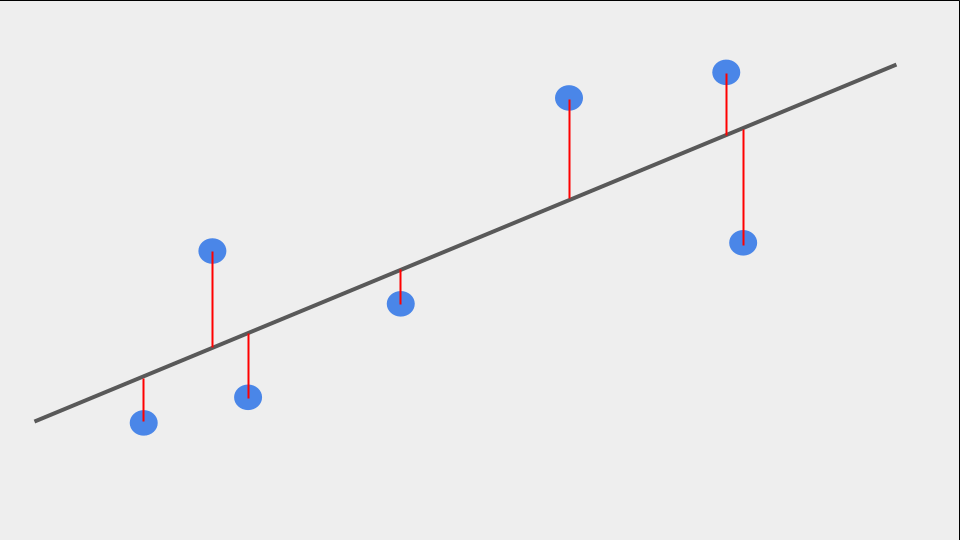
\includegraphics[width=0.7\textwidth]{SSD.png}
    \centering
    \caption{Adding the (squared) lengths of the red lines will tell us
    how good this fit is.}
    \label{fig:ssd}
\end{figure}

\subsection{Rewrite the problem using linear algebra}

It might seem strange to do this now, but it will help us find a solution
to the problem and help us use the technique when we have many input
and/or output variables.

First, let's stack the $y_i$ in a vector.
\begin{equation}
    \begin{bmatrix}
        y_1  \\
        y_2 \\
        \vdots \\
        y_N
    \end{bmatrix}
\end{equation}

Next, convince yourself that if we can write a vector of function
predictions like this:

\begin{equation}
    \begin{bmatrix}
        \hat{y}_1  \\
        \hat{y}_2 \\
        \vdots \\
        \hat{y}_N
    \end{bmatrix}
    = 
    \begin{bmatrix}
        x_1 & 1 \\
        x_2 & 1 \\
        \vdots \\
        x_N & 1
    \end{bmatrix}
    \begin{bmatrix}
        a \\ b
    \end{bmatrix}
\end{equation}



%\subsection{Finding the solution}

%\section{ Multi-variable linear regression }

%\section{ Polynomial regression }

%\section{ General regression }



\end{document}
